\documentclass[a4paper,12pt]{report}
\usepackage[top=1cm, left=1cm, right=1cm, bottom=1.5cm, landscape]{geometry}
\usepackage[T1]{fontenc}
\usepackage{hyperref,graphicx,amsmath,pdfpages,float,subfig,enumitem,lastpage}
\usepackage{longtable}


\begin{document}
\begin{center}
    \large \textbf{CHE613A: The Structure \& Rheology Of Complex Fluids\\(Assignment 5)}
\end{center}

\begin{flushright}
    \textit{\underline{Submitted by}}\\Keerthi Vasan M\\Roll No.: 21102023\\keerthi21@iitk.ac.in\\ \today
\end{flushright}
\vspace{-5mm}
\rule{\textwidth}{0.5 pt}
\noindent
\textbf{Question: }Fit a multimode Maxwell model with modulus and relaxation time scales G$_i$ and $\tau_i$ (i = 1 to N) to the given experimental plot of G' and G'' versus $\omega$. Obtain an expression for relaxation modulus G(t) and plot it with respect to time. Also calculate the shear viscosity $\eta$.\\[0.4 cm]
\textbf{Solution:} As the first part the problem the given plot is used to extract the data using the data extraction software \textbf{WebPlotDigitizer}. The given plot of G' and G'' versus $\omega$ is shown below:
\begin{figure}[H]%
    \centering
    \subfloat{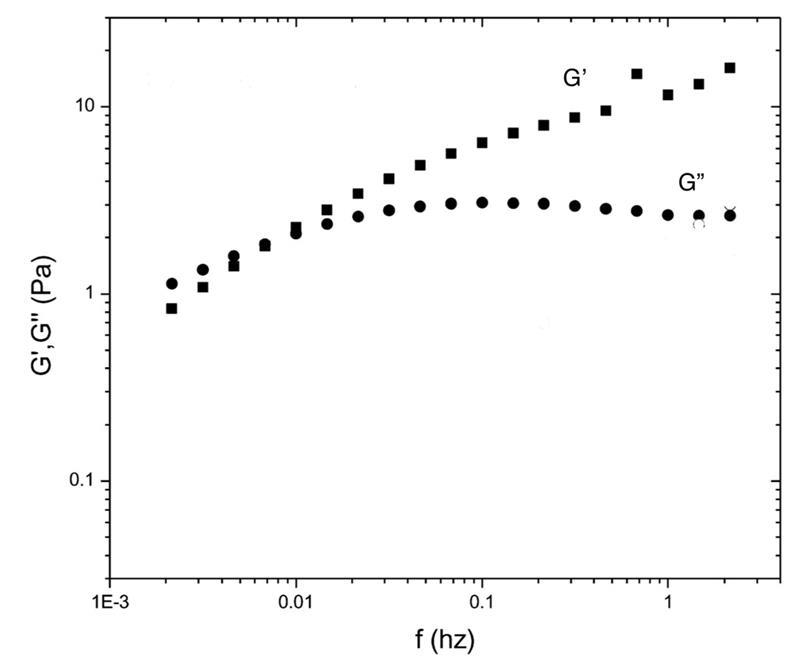
\includegraphics[scale=0.4]{Plot.png}}%
    \qquad
    \subfloat{{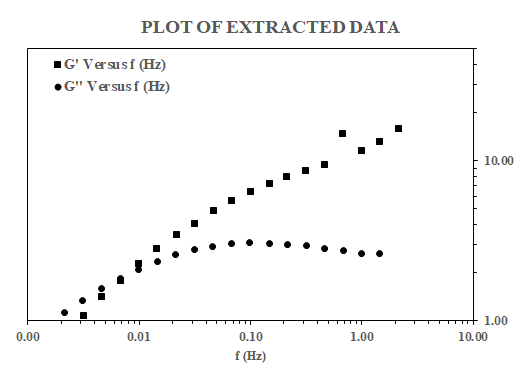
\includegraphics[scale=0.8]{Extracted.png} }}%
\end{figure}
\noindent
Now, data obtained from the \textbf{WebPlotDigitizer} is then plotted to verify the visual accuracy of the extracted data. From the above figures, it can be concluded that the extracted data reasonably fits the actual graph given in the question. Corresponding extracted data (G', G'', f) are given in the table  below:
% Please add the following required packages to your document preamble:
% \usepackage{longtable}
% Note: It may be necessary to compile the document several times to get a multi-page table to line up properly
% Please add the following required packages to your document preamble:
% \usepackage{graphicx}
\begin{table}[H]
\resizebox{\textwidth}{!}{%
\begin{tabular}{|c|c|c|c|c|c|c|c|c|c|c|c|c|c|c|c|c|c|c|}
\hline
\textbf{f (hz)} &
  0.0031 &
  0.0046 &
  0.0068 &
  0.0099 &
  0.0145 &
  0.0216 &
  0.0314 &
  0.0462 &
  0.0681 &
  0.1003 &
  0.1478 &
  0.2122 &
  0.3127 &
  0.4607 &
  0.6744 &
  1.0000 &
  1.4544 &
  2.1568 \\ \hline
\textbf{G'} &
  1.0834 &
  1.4177 &
  1.7969 &
  2.2774 &
  2.8134 &
  3.4534 &
  4.0792 &
  4.8804 &
  5.6189 &
  6.3868 &
  7.1673 &
  7.9407 &
  8.6857 &
  9.5005 &
  14.8752 &
  11.5872 &
  13.1708 &
  15.9610 \\ \hline
\textbf{f (hz)} &
  0.0021 &
  0.0031 &
  0.0046 &
  0.0067 &
  0.0099 &
  0.0146 &
  0.0213 &
  0.0316 &
  0.0459 &
  0.0677 &
  0.0990 &
  0.1469 &
  0.2150 &
  0.3167 &
  0.4607 &
  0.6787 &
  0.9936 &
  1.4544 \\ \hline
\textbf{G''} &
  1.1330 &
  1.3469 &
  1.6012 &
  1.8435 &
  2.0955 &
  2.3515 &
  2.5887 &
  2.7955 &
  2.9236 &
  3.0382 &
  3.0774 &
  3.0382 &
  2.9995 &
  2.9424 &
  2.8497 &
  2.7423 &
  2.6389 &
  2.6389 \\ \hline
\end{tabular}%
}
\end{table}
\newpage
\noindent\textbf{Steps followed:}
\begin{itemize}
    \item I am using MATLAB for the this assignment 05.
    \item The number of Maxwell mode (N) that I am going to use is first fixed.
    \item Then convert the extracted frequency data (f (Hz)) into corresonding angular frequency using the relationship $\omega=2\pi f$.
    \item Now, the relaxation time of the each mode is found using the relationship given to us. $\tau_i=\tau_{min}\times \big(\frac{\tau_{max}}{\tau_{min}}\big)^{\left( \frac{i=1}{N-1} \right)}$ where $i=1,2,3,....N$ and $\tau_{min}=1/\omega_{max}$ and $\tau_{max}=1/\omega_{min}$.
    \item ($\omega$,G') data extracted from the given graph is used to find the relaxation modulus of each Maxwell mode (g$_i$ where $i=1,2,...N$) using the relation $G'(\omega)=\sum_{i=1}^N \frac{g_i\omega^2\tau_i^2}{1+\omega^2\tau_i^2}$.
    \item Now, for each mode `i' calculate the term $\frac{\omega^2\tau_i^2}{1+\omega^2\tau_i^2}$ for different values of $\omega$ and store it as a row in a matrix variable called ``abscissa''. So, i$^{th}$ row of the matrix ``abscissa'' gives all the i$^{th}$ mode's $\frac{\omega^2\tau_i^2}{1+\omega^2\tau_i^2}$ value. Also note that, each column of any i$^{th}$ row of the matrix ``abscissa'' denotes the value of $\frac{\omega^2\tau_i^2}{1+\omega^2\tau_i^2}$ corresponding to different $\omega$.
    \item Therefore, ``abscissa(n,:)'' denotes the entire row of the matrix ``abscissa" corresponding to the mode `n'. 
    \item Now, using the extracted G$'(\omega)$ data and the ``abscissa'' matrix we can calculate the relaxation modulus of each Maxwell mode (g$_i$ where $i=1,2,...N$) using the relation $G'(\omega)=\sum_{i=1}^N \frac{g_i\omega^2\tau_i^2}{1+\omega^2\tau_i^2}$. For this purpose, I have used the ``lsqcurvefit'' Matlab function.
    \item Giving a initial guess value of one for relaxation modulus of each mode, ``lsqcurvefit'' Matlab function determines the actual relaxation time of each `N' mode. Termination tolerance while doing the curve fitting is set at $e^{\pi/2}$ using the ``options'' statement of ``lsqcurvefit'' Matlab function. 
    \item If any mode's relaxation modulus found is negative then the `N' chosen is reduced and all the above procedure are repeated. Repeat the procedure till the relaxation modulus of each mode is positive.
    \item Once the relaxation modulus of each mode is found, it is then used to find G"($\omega$) data for each $\omega$. Cross checking the ,thus found, G"($\omega$) with the G"($\omega$) that is extracted will shows accuracy of the ``lsqcurvefit'' fit that is done earlier to find the relaxation modulus of each mode. Plot the ($\omega$,G"($\omega$)) calculated and ($\omega$,G"($\omega$)) that is extracted and see how well the both plot fit each other. Change the `N' till error in the G"($\omega$) calculated is minimum.
    \item Obtain the expression for overall relaxation modulus and shear viscosity in terms of time, relaxation modulus of each mode and relaxation time of each mode. We know that for a multimode Maxwell model $G(t)=\sum_{m=1}^N g_m exp\big(\frac{-t}{\tau_m}\big)$ and $\eta(t)=\sum_{m=1}^N\eta_m=\sum_{m=1}^N\tau_mG(\omega)=\sum_{m=1}^N g_m\tau_mexp\big(\frac{-t}{\tau_m}\big)$.
\end{itemize}
\textbf{Full algorithm used in the Matlab is provided below:}
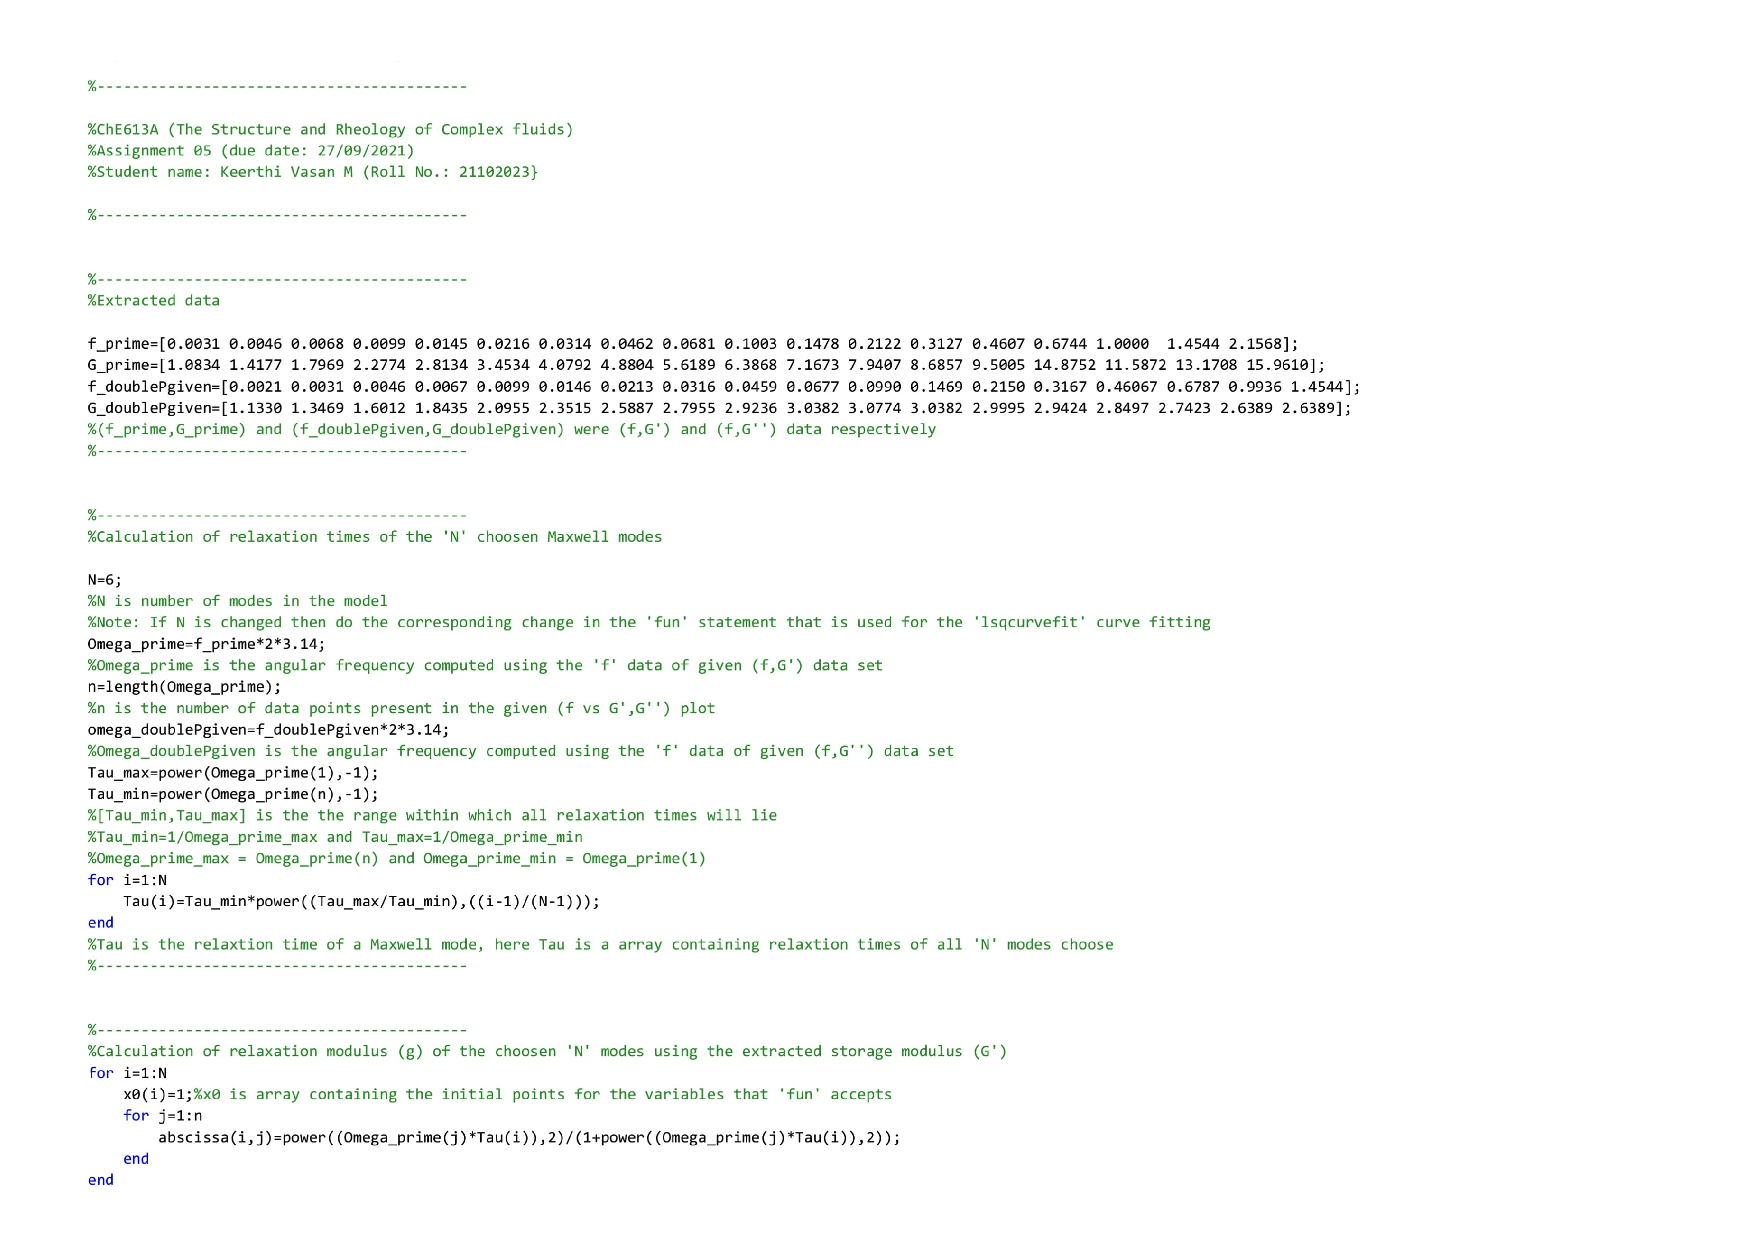
\includepdf[pages=-,pagecommand={},fitpaper=true]{first.pdf}
\noindent
\textbf{Running the above Matlab program gives the following output}:\\
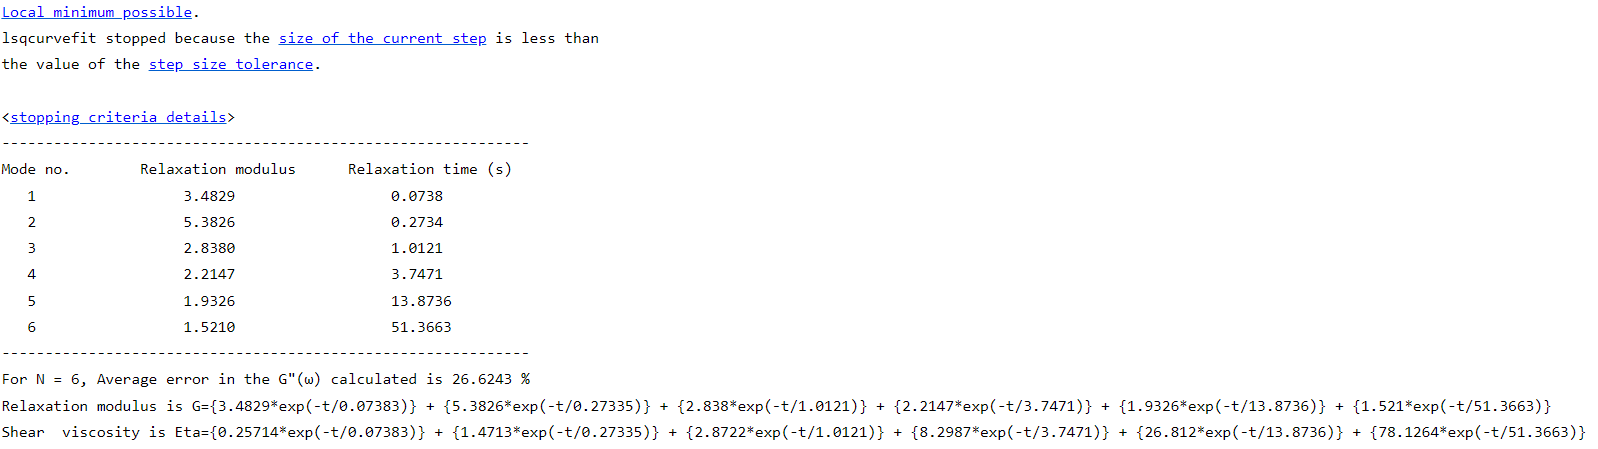
\includegraphics[scale=0.8]{Results.png}
\begin{figure}[H]%
    \centering
    \subfloat{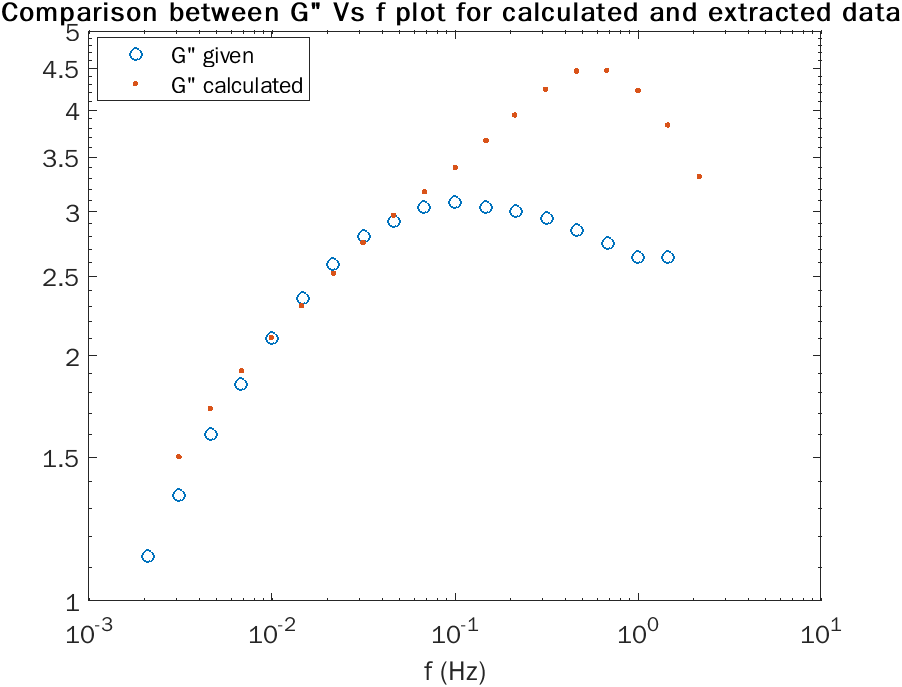
\includegraphics[scale=0.85]{Comparison_Plot.png}}%
    \qquad
    \subfloat{{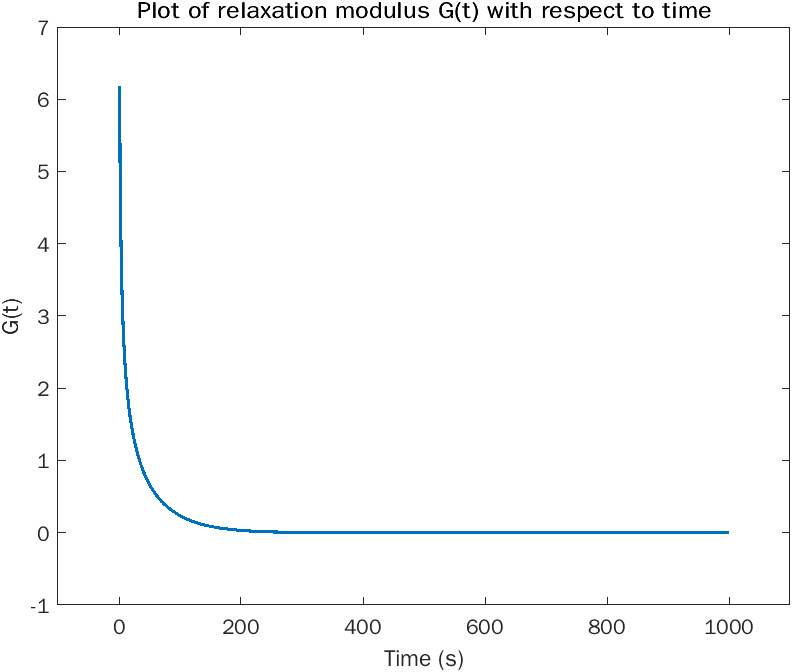
\includegraphics[scale=0.8]{Relaxation_Plot.png} }}%
\end{figure}
\newpage

\noindent \textbf{Reason for the choice of `N' and other observations}\\
Following table shows the model results for various values of `N' and its corresponding relaxation modulus and time of each `N' modes. Average value of all the error in calculated G$''(\omega)$ is also computed for each choice of `N'. It is calculated as  $\Bigg\{\frac{1}{n}\sum_{i=1}^n\bigg(\frac{|G"_{\text{extracted},i}(\omega)-G"_{\text{calculated},i}(\omega)|}{G"_{\text{extracted},i}(\omega)}\bigg)\Bigg\}$ where `n' is the number of data points present in the given (f vs G$'$,G$''$) plot.
\begin{table}[H]
\resizebox{\textwidth}{!}{%
\begin{tabular}{|c|c|c|c|c|c|c|c|c|c|c|c|c|c|c|c|c|c|c|c|c|c|c|c|c|c|c|c|}
\hline
N    & \multicolumn{2}{c|}{2} & \multicolumn{3}{c|}{3} & \multicolumn{4}{c|}{4} & \multicolumn{5}{c|}{5} & \multicolumn{6}{c|}{6} & \multicolumn{7}{c|}{7}    \\ \hline
\begin{tabular}[c]{@{}c@{}}Average error \% of all \\ computed G"($\omega$)\end{tabular} &
  \multicolumn{2}{c|}{104.2945} &
  \multicolumn{3}{c|}{39.2427} &
  \multicolumn{4}{c|}{31.2706} &
  \multicolumn{5}{c|}{26.9427} &
  \multicolumn{6}{c|}{26.6243} &
  \multicolumn{7}{c|}{30.0927} \\ \hline
Mode & 1          & 2         & 1      & 2     & 3     & 1    & 2   & 3   & 4   & 1  & 2  & 3  & 4  & 5  & 1  & 2 & 3 & 4 & 5 & 6 & 1 & 2 & 3 & 4 & 5 & 6 & 7 \\ \hline
Relaxation modulus, g$_i$ &
  24.4339 &
  5.757 &
  12.0952 &
  7.3449 &
  2.5 &
  7.7888 &
  6.1849 &
  3.4581 &
  2.0537 &
  4.288 &
  6.3312 &
  2.5565 &
  2.7899 &
  1.6278 &
  3.3144 &
  5.6098 &
  2.5231 &
  2.5965 &
  1.5966 &
  1.6556 &
  7.0761 &
  0.0323 &
  7.3678 &
  -1.9004 &
  4.8717 &
  -0.4916 &
  2.1058 \\ \hline
Relaxation time (s) &
  0.0738 &
  51.3663 &
  0.0738 &
  1.9474 &
  51.3663 &
  0.0738 &
  0.6542 &
  5.7969 &
  51.3663 &
  0.0738 &
  0.3792 &
  1.9474 &
  10.0015 &
  51.3663 &
  0.0738 &
  0.2734 &
  1.0121 &
  3.7471 &
  13.8736 &
  51.3663 &
  0.0738 &
  0.2198 &
  0.6542 &
  1.9474 &
  5.7969 &
  17.2559 &
  51.3663 \\ \hline
\end{tabular}%
}
\end{table}

\begin{itemize}
    \item As `N' is increased starting from 2, the average error is decreasing significantly starting from 104.2945\% (for N=2) to 26.6243\% (for N=6). \textit{Note:} N=7 is special case which is discussed in the upcoming points.
    \item Ideal `N' to choose is the one that have least average error in the G$''(\omega)$ calculated using $G''(\omega)=\sum_{i=1}^N \frac{g_i\ \omega\ \tau_i}{1+\omega^2\tau_i^2}$ relation of multimode Maxwell model (where g$_i$ $(i=1,2,...N)$ are obtained by curve fitting using ``lsqcurvefit'').
    \item When N=7, some of the relaxation modulus of the modes (g$_i$) were negative showing that for the given plot (shown in page 1) N=7 leads to over fitting. It is better restrict N to be less than 7. Also note that the error percentage is increasing to 30.0927\% (for N=7) from 26.6243\% (for N=6). So, N=6 is ideal value of number of modes to be used in the model.
    \item When N=6, model results are as follows (also shown in page 6):\\[0.35cm]
    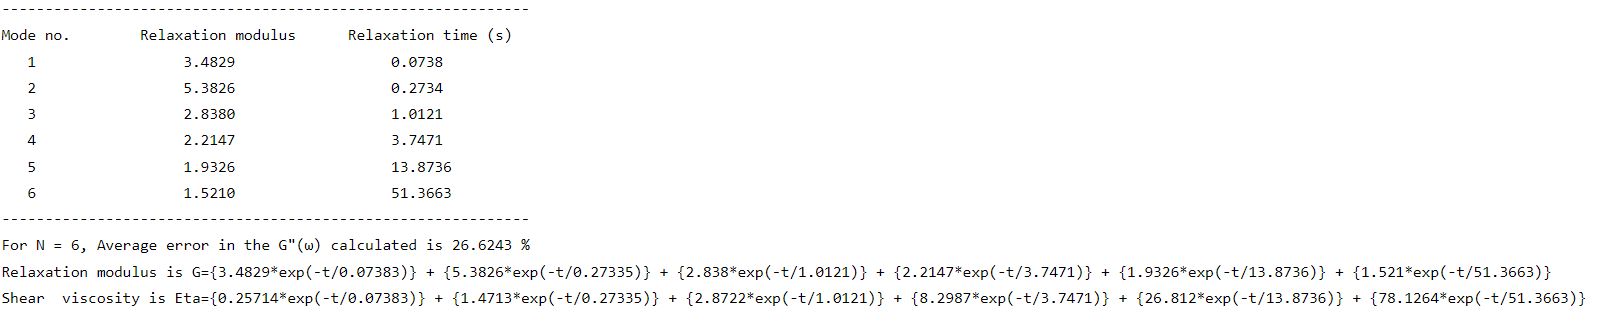
\includegraphics[scale=0.75]{Results_Conclusion.png}
    \\[0.35cm]Plot of overall relaxation modulus of `N' mode Maxwell model (G(t)) versus time is shown in page 6.
\end{itemize}
\end{document}
